%%%%%%%%%%%%%%%%%%%%%%%%%%%%%%%%%%%%%%%%%
% Masters/Doctoral Thesis 
% LaTeX Template
% Version 2.5 (27/8/17)
%
% This template was downloaded from:
% http://www.LaTeXTemplates.com
%
% Version 2.x major modifications by:
% Vel (vel@latextemplates.com)
%
% This template is based on a template by:
% Steve Gunn (http://users.ecs.soton.ac.uk/srg/softwaretools/document/templates/)
% Sunil Patel (http://www.sunilpatel.co.uk/thesis-template/)
%
% Template license:
% CC BY-NC-SA 3.0 (http://creativecommons.org/licenses/by-nc-sa/3.0/)
%
%%%%%%%%%%%%%%%%%%%%%%%%%%%%%%%%%%%%%%%%%

%----------------------------------------------------------------------------------------
%	PACKAGES AND OTHER DOCUMENT CONFIGURATIONS
%----------------------------------------------------------------------------------------

\documentclass[
11pt, % The default document font size, options: 10pt, 11pt, 12pt
%oneside, % Two side (alternating margins) for binding by default, uncomment to switch to one side
english, % ngerman for German
singlespacing, % Single line spacing, alternatives: onehalfspacing or doublespacing
%draft, % Uncomment to enable draft mode (no pictures, no links, overfull hboxes indicated)
%nolistspacing, % If the document is onehalfspacing or doublespacing, uncomment this to set spacing in lists to single
%liststotoc, % Uncomment to add the list of figures/tables/etc to the table of contents
%toctotoc, % Uncomment to add the main table of contents to the table of contents
%parskip, % Uncomment to add space between paragraphs
%nohyperref, % Uncomment to not load the hyperref package
headsepline, % Uncomment to get a line under the header
%chapterinoneline, % Uncomment to place the chapter title next to the number on one line
%consistentlayout, % Uncomment to change the layout of the declaration, abstract and acknowledgements pages to match the default layout
onecolumn
]{MastersDoctoralThesis} % The class file specifying the document structure



\usepackage[utf8]{inputenc} % Required for inputting international characters
\usepackage[T1]{fontenc} % Output font encoding for international characters

\usepackage{mathpazo} % Use the Palatino font by default
\usepackage{graphicx}
\usepackage{subfig}
\usepackage{transparent}
\usepackage{eso-pic}
\usepackage[en-US]{datetime2}
\usepackage{tikz}




\usepackage[round]{natbib}   % omit 'round' option if you prefer square brackets
%\usepackage{csquotes}
\usepackage[autostyle=true]{csquotes} % Required to generate language-dependent quotes in the bibliography

%\usepackage{wrapfig} % text around figure
% \usepackage[section]{placeins} % force figures to their respective sections
%\usepackage{placeins} % force figures to appear before a barier

\usepackage{enumitem} % listing and labeling items like research questions
\usepackage[nottoc,notlot,notlof]{tocbibind} % adds the bibliography to the table of contents
\usepackage{xcolor} %highlight text
\usepackage{float}
\usepackage{lmodern,textcomp} %euro symbol
\usepackage{textcomp} % text registeres
% combining subfigures
%\usepackage{subcaption}
%\usepackage[labelformat=parens,labelsep=quad,skip=3pt]{caption}
%\usepackage{graphicx} 
%\usepackage{fixltx2e}
%\usepackage{cases}
\usepackage{hyperref, amsmath,cleveref}
\DeclareMathOperator*{\argmax}{argmax} % thin space, limits underneath in displays

\usepackage{fontspec}
\defaultfontfeatures{Mapping=tex-text}
\setmainfont{Garamond}


\usepackage{multicol}
\usepackage{caption}
\captionsetup{justification=justified,singlelinecheck=false}
\usepackage{makecell}
\usepackage[htt]{hyphenat}
\usepackage{booktabs}

\usepackage{scrextend}
%\usepackage{microtype}

% Define how long words will be hyphenated
\hyphenation{Niederschlags-ereignisses}
\hyphenation{Nieder-schlags-radare}
\hyphenation{Nieder-schlag}
\hyphenation{Überlappungs-bereich}
\hyphenation{Hangrut-schungen}
\hyphenation{Des-weiteren}

\newcommand{\blankpage}{
\newpage
\thispagestyle{empty}
\mbox{}
\newpage
}

%% Coverpage image
%\usepackage{eso-pic}
%\newcommand\BackgroundPic{%
%\put(0,0){%
%\parbox[b][\paperheight]{\paperwidth}{%
%%\vfill
%\vspace{12.7cm}
%\centering
%\includegraphics[width=\paperwidth,%
%keepaspectratio]{radar3d_a.png}%
%\vfill
%}}}

%% End page image
%\usepackage{eso-pic}
%\newcommand\LastCoverPic{%
%\put(0,0){%
%\parbox[b][\paperheight]{\paperwidth}{%
%%\vfill
%\vspace{0cm}
%\centering
%\includegraphics[width=\paperwidth,%
%keepaspectratio]{radar3d_a.png}%
%\vfill
%}}}
%%----------------------------------------------------------------------------------------
%	MARGIN SETTINGS
%----------------------------------------------------------------------------------------

\geometry{
	paper=a4paper, % Change to letterpaper for US letter
	inner=1.5cm, % Inner margin
	outer=1.5cm, % Outer margin
	bindingoffset=1cm, % Binding offset
	top=1.5cm, % Top margin
	bottom=1.5cm, % Bottom margin
	columnsep=0.75cm
	%showframe, % Uncomment to show how the type block is set on the page
}

%----------------------------------------------------------------------------------------
%	THESIS INFORMATION
%----------------------------------------------------------------------------------------

\thesistitle{This is the title of my dissertation
} % Your thesis title, this is used in the title and abstract, print it elsewhere with \ttitle
\supervisor{Name \textsc{LastName}, Ph.D. \\* Prof. Dr. Name \textsc{LastName}} % Your supervisor's name, this is used in the title page, print it elsewhere with \supname
\degree{Doctor of Philosophy} % Your degree name, this is used in the title page and abstract, print it elsewhere with \degreename
\author{MyName \textsc{MyLastName}} % Your name, this is used in the title page and abstract, print it elsewhere with \authorname
\addresses{} % Your address, this is not currently used anywhere in the template, print it elsewhere with \addressname

\subject{Natural Hazards} % Your subject area, this is not currently used anywhere in the template, print it elsewhere with \subjectname
\keywords{} % Keywords for your thesis, this is not currently used anywhere in the template, print it elsewhere with \keywordnames
\university{\href{http://www.uni-potsdam.de}{University of Potsdam}} % Your university's name and URL, this is used in the title page and abstract, print it elsewhere with \univname
\department{\href{https://www.uni-potsdam.de/umwelt/}{Institute of Environmental Science and Geography}} % Your department's name and URL, this is used in the title page and abstract, print it elsewhere with \deptname
\group{\href{https://www.uni-potsdam.de/de/umwelt/forschung/ag-hydrologie-und-klimatologie.html}{Geoecology}} % Your research group's name and URL, this is used in the title page, print it elsewhere with \groupname
\faculty{\href{http://www.uni-potsdam.de/mnfakul/}{Faculty of Science}} % Your faculty's name and URL, this is used in the title page and abstract, print it elsewhere with \facname

\AtBeginDocument{
\hypersetup{pdftitle=\ttitle} % Set the PDF's title to your title
\hypersetup{pdfauthor=\authorname} % Set the PDF's author to your name
\hypersetup{pdfkeywords=\keywordnames} % Set the PDF's keywords to your keywords
}

\begin{document}
%\AddToShipoutPicture*{\BackgroundPic} % to place the background image only in the cover page

\frontmatter % Use roman page numbering style (i, ii, iii, iv...) for the pre-content pages

\pagestyle{plain} % Default to the plain heading style until the thesis style is called for the body content

%----------------------------------------------------------------------------------------
%	TITLE PAGE
%----------------------------------------------------------------------------------------

\begin{titlepage}
\begin{center}


%\begin{figure}
%%\vspace*{.06\textheight}
%    \centering
%\subfloat{\includegraphics[width=3cm]{Mathnatlogo.eps}}
%  \hfill
%\subfloat{\includegraphics[width=3cm]{Logo_Inst.jpg}}
%\end{figure}

%\begin{figure}[!tbp]
%  \centering
%  \begin{minipage}[b]{0.2\textwidth}
%    \includegraphics[width=\textwidth]{Mathnatlogo.eps}
%  \end{minipage}
%  \hfill
%  \begin{minipage}[b]{0.2\textwidth}
%    \includegraphics[width=\textwidth]{Mathnatlogo.eps}
%  \end{minipage}
%\end{figure}


\vspace*{2cm}
{\scshape\LARGE \univname\par}\vspace{1.5cm} % University name

\textsc{\Large Cumulative Dissertation}\\[0.4cm] % Thesis type

\HRule \\[0.3cm] % Horizontal line
{\huge \bfseries {\ttitle}\par}\vspace{0.4cm} % Thesis title
\HRule \\[0.3cm] % Horizontal line

\vspace*{1.5cm}

by\\
\vspace{0.8cm}
{\Large \textbf{\authorname}}

\vspace*{2cm}

Supervisors:\\
\supname
 
\vspace{3cm}
%\vspace*{\fill}
%\mbox{}


\large for the degree of\\
doctor rerum naturalium (Dr. rer. nat.)\\ % University requirement text
in \groupname\\\deptname\\\facname\\ % Research group name and department name
 
\bigskip

{\large April 2019}\\[4cm] % Date
%\includegraphics{Logo} % University/department logo - uncomment to place it

\end{center}
\end{titlepage}

%----------------------------------------------------------------------------------------
%	COMMITTEE
%----------------------------------------------------------------------------------------

\begin{committee}
\begin{center}

{\Large \bfseries \ttitle\par}\vspace{0.4cm} % Thesis title


by \authorname\\

\vfill
 
\begin{minipage}[t]{0.43\textwidth}
\begin{flushleft} \large
\emph{Supervisor:}\\
\vspace{\baselineskip}
Name LastName, Ph.D. (\textit{Reviewer})\\
\end{flushleft}
\end{minipage}
\begin{minipage}[t]{0.56\textwidth}
\begin{flushright} \large
\emph{Affiliation:}\\
\vspace{\baselineskip}
\textit{University of Potsdam}\\ 
\end{flushright}
\end{minipage}

\bigskip

\begin{minipage}[t]{0.43\textwidth}
\begin{flushleft} \large
\emph{Co-Supervisor:}\\
\vspace{\baselineskip}
Prof. Dr. Name LastName (\textit{Reviewer})\\
\end{flushleft}
\end{minipage}
\begin{minipage}[t]{0.56\textwidth}
\begin{flushright} \large
\emph{} \\
\vspace{\baselineskip}
\textit{University of Potsdam}\\ 
\end{flushright}
\end{minipage}

\bigskip
%\bigskip

\begin{minipage}[t]{0.43\textwidth}
\begin{flushleft} \large
\emph{Mentor:}\\
\vspace{\baselineskip}
Prof. Name LastName, Ph.D.
\end{flushleft}
\end{minipage}
\begin{minipage}[t]{0.56\textwidth}
\begin{flushright} \large
\vspace{\baselineskip}
\textit{University of Potsdam}
\end{flushright}
\end{minipage}

\vfill

\vfill

\begin{minipage}[t]{0.47\textwidth}
\begin{flushleft} \large
\emph{Assessment Committee:}\\
\vspace{\baselineskip}
Prof. Name LastName, Ph.D. \textit{(Chair)}\\
\vspace{\baselineskip}
Prof. Dr. Name LastName\\
\vspace{\baselineskip} 
Prof. Dr. Name LastName\\
\vspace{\baselineskip} 
Prof. Dr. Name LastName (\textit{Reviewer})\\

\end{flushleft}
\end{minipage}
\begin{minipage}[t]{0.52\textwidth}
\begin{flushright} \large
\emph{} \\
\vspace{\baselineskip}
\textit{University of Potsdam}\\
\vspace{\baselineskip}
\textit{University of Potsdam}\\ 
\vspace{\baselineskip} 
\textit{University of Potsdam}\\
\vspace{\baselineskip} 
\textit{Wageningen University and Research, Netherlands}\\

\end{flushright}
\end{minipage}

\end{center}
 
\vfill
\noindent
\large \textit{Publication-based dissertation submitted in fulfilment of the requirements for the degree of \degreename\ under the discipline of \groupname\ in the \deptname\, \facname\ at the \univname.}
 
%\vfill

\end{committee}

%----------------------------------------------------------------------------------------
%	DECLARATION PAGE
%----------------------------------------------------------------------------------------

\onecolumn %% allow single column for first pages

\begin{declaration}
\addchaptertocentry{\authorshipname} % Add the declaration to the table of contents
\noindent I, \authorname, declare that this thesis titled, \enquote{\ttitle} and the work presented in it are my own. I confirm that:

\begin{itemize} 
\item This work was done wholly or mainly while in candidature for a research degree at the \univname.
\item Where any part of this dissertation has previously been submitted for a degree or any other qualification at the \univname, or any other institution, this has been clearly stated.
\item Where I have consulted the published work of others, this is always clearly attributed.
\item Where I have quoted from the work of others, the source is always given. With the exception of such quotations, this thesis is entirely my own work.
\item I have acknowledged all main sources of help.
\item Where the thesis is based on work done by myself jointly with others, I have made clear exactly what was done by others and what I have contributed myself.\\
\end{itemize}
 
\vspace*{.02\textheight}

\noindent Signature:\\
\rule[0.5em]{25em}{0.5pt} % This prints a line for the signature

\vspace*{.02\textheight} 
\noindent Date:\\
\rule[0.5em]{25em}{0.5pt} % This prints a line to write the date
\end{declaration}

\cleardoublepage

%----------------------------------------------------------------------------------------
%	QUOTATION PAGE
%----------------------------------------------------------------------------------------

\vspace*{0.2\textheight}
\begin{flushright}
\noindent\enquote{\itshape Sometimes attaining the deepest familiarity with a question is our best substitute for actually having the answer.}\medskip
\end{flushright}
\hfill \textsc{Brian Greene}

%----------------------------------------------------------------------------------------
%	ABSTRACT PAGE
%----------------------------------------------------------------------------------------

\begin{addmargin}[4.7em]{3.5em} % add margins on both sides of abstract. Narrower looks nicer, imho

\begin{abstract}
\label{abstract}
\addchaptertocentry{\abstractname} % Add the abstract to the table of contents
\setlength{\parskip}{1em} % give extra space between paragraphs
\noindent

Lorem ipsum dolor sit amet, consectetur adipiscing elit. Nunc varius commodo lectus ut ultricies. Curabitur pellentesque laoreet auctor. Proin nec ornare sem. Sed pellentesque augue tortor, in faucibus massa auctor quis. Cras scelerisque, leo quis faucibus euismod, lectus mi sodales enim, et cursus quam elit at eros. Phasellus dapibus vitae dui in malesuada. Vestibulum sed ex ac lectus pretium dapibus. Sed aliquet blandit urna ut lobortis. Phasellus orci nunc, varius et nulla nec, blandit fermentum nulla.

Fusce aliquet mauris sed interdum ultricies. Nunc rutrum viverra risus, ac congue urna vulputate malesuada. Fusce euismod sollicitudin lorem at varius. Aenean lacinia quam tortor, accumsan congue velit ullamcorper in. In dignissim sed magna sit amet ultrices. Nulla at tincidunt mi. Praesent fermentum risus quis tellus commodo feugiat. Proin et posuere eros. Suspendisse consectetur sapien lectus, non rhoncus elit tristique vitae. Vivamus nec finibus sapien, id laoreet lacus. Aliquam vehicula lectus vitae porta hendrerit. Aliquam scelerisque sit amet lorem nec eleifend. Donec egestas quam in lacus convallis, id dictum massa porta. Donec tincidunt rhoncus diam eget sodales.

Maecenas lobortis urna mattis pretium mattis. Nullam a scelerisque odio. Maecenas tincidunt euismod hendrerit. In hac habitasse platea dictumst. Nulla porttitor pulvinar est et sagittis. Nam porttitor mattis erat, ac tempus ligula congue quis. Praesent mattis libero sit amet nunc fringilla tincidunt. In convallis tellus non sem vulputate rutrum. Integer vestibulum leo a lectus porttitor bibendum. Phasellus fermentum, massa et sodales consequat, lectus ipsum ultricies enim, vitae maximus sapien ligula eget sapien. Nunc eget sem feugiat, laoreet tortor vel, mollis ipsum. Donec nisi turpis, hendrerit a porta ut, tristique accumsan nibh. Donec nec vehicula orci.

Quisque nisl felis, vulputate vel lectus a, porttitor sagittis nunc. Maecenas interdum, ex id maximus egestas, velit sapien scelerisque ex, sit amet rutrum elit ex ac nibh. Sed dapibus sapien velit. Pellentesque habitant morbi tristique senectus et netus et malesuada fames ac turpis egestas. Sed mollis nisl euismod tempus venenatis. Suspendisse elementum ante id lorem elementum, sit amet dictum mi posuere. Suspendisse potenti. Phasellus dui urna, ultrices in vehicula ut, aliquet ac quam. Quisque aliquet fermentum nunc, nec laoreet lacus vulputate nec. Nullam gravida vel nibh a tincidunt. Fusce a auctor est. Curabitur lectus nulla, lobortis non dui ut, tincidunt fringilla purus. Donec dapibus arcu vel turpis feugiat pulvinar. Pellentesque volutpat enim tincidunt lacinia venenatis. Vivamus justo leo, feugiat eget felis quis, fermentum consectetur turpis.

Vestibulum tincidunt ipsum turpis. Vivamus et nulla sit amet nisl egestas volutpat et eget est. Duis quis sapien vel est fermentum auctor. Quisque volutpat mollis leo in rhoncus. Ut rutrum ligula sed erat molestie, nec tristique dui malesuada. Ut bibendum, eros quis placerat euismod, metus sem rhoncus purus, vel interdum massa risus vitae libero. Integer et imperdiet nibh. Donec venenatis turpis in vehicula dapibus. Nullam luctus porttitor ex, nec cursus nunc semper non. Nam iaculis ligula ut quam feugiat ultricies. Aliquam a blandit massa. Nunc eget ipsum mauris.

\end{abstract}

\end{addmargin}

%----------------------------------------------------------------------------------------
%	ZUSAMMENFASSUNG PAGE
%----------------------------------------------------------------------------------------
\begin{addmargin}[4.2em]{2.5em}
\begin{zusammenfassung}
\addchaptertocentry{\zusammenfassungsname} % Add the abstract to the table of contents


\noindent

Lorem ipsum dolor sit amet, consectetur adipiscing elit. Nunc varius commodo lectus ut ultricies. Curabitur pellentesque laoreet auctor. Proin nec ornare sem. Sed pellentesque augue tortor, in faucibus massa auctor quis. Cras scelerisque, leo quis faucibus euismod, lectus mi sodales enim, et cursus quam elit at eros. Phasellus dapibus vitae dui in malesuada. Vestibulum sed ex ac lectus pretium dapibus. Sed aliquet blandit urna ut lobortis. Phasellus orci nunc, varius et nulla nec, blandit fermentum nulla.

Fusce aliquet mauris sed interdum ultricies. Nunc rutrum viverra risus, ac congue urna vulputate malesuada. Fusce euismod sollicitudin lorem at varius. Aenean lacinia quam tortor, accumsan congue velit ullamcorper in. In dignissim sed magna sit amet ultrices. Nulla at tincidunt mi. Praesent fermentum risus quis tellus commodo feugiat. Proin et posuere eros. Suspendisse consectetur sapien lectus, non rhoncus elit tristique vitae. Vivamus nec finibus sapien, id laoreet lacus. Aliquam vehicula lectus vitae porta hendrerit. Aliquam scelerisque sit amet lorem nec eleifend. Donec egestas quam in lacus convallis, id dictum massa porta. Donec tincidunt rhoncus diam eget sodales.

Maecenas lobortis urna mattis pretium mattis. Nullam a scelerisque odio. Maecenas tincidunt euismod hendrerit. In hac habitasse platea dictumst. Nulla porttitor pulvinar est et sagittis. Nam porttitor mattis erat, ac tempus ligula congue quis. Praesent mattis libero sit amet nunc fringilla tincidunt. In convallis tellus non sem vulputate rutrum. Integer vestibulum leo a lectus porttitor bibendum. Phasellus fermentum, massa et sodales consequat, lectus ipsum ultricies enim, vitae maximus sapien ligula eget sapien. Nunc eget sem feugiat, laoreet tortor vel, mollis ipsum. Donec nisi turpis, hendrerit a porta ut, tristique accumsan nibh. Donec nec vehicula orci.

Quisque nisl felis, vulputate vel lectus a, porttitor sagittis nunc. Maecenas interdum, ex id maximus egestas, velit sapien scelerisque ex, sit amet rutrum elit ex ac nibh. Sed dapibus sapien velit. Pellentesque habitant morbi tristique senectus et netus et malesuada fames ac turpis egestas. Sed mollis nisl euismod tempus venenatis. Suspendisse elementum ante id lorem elementum, sit amet dictum mi posuere. Suspendisse potenti. Phasellus dui urna, ultrices in vehicula ut, aliquet ac quam. Quisque aliquet fermentum nunc, nec laoreet lacus vulputate nec. Nullam gravida vel nibh a tincidunt. Fusce a auctor est. Curabitur lectus nulla, lobortis non dui ut, tincidunt fringilla purus. Donec dapibus arcu vel turpis feugiat pulvinar. Pellentesque volutpat enim tincidunt lacinia venenatis. Vivamus justo leo, feugiat eget felis quis, fermentum consectetur turpis.

Vestibulum tincidunt ipsum turpis. Vivamus et nulla sit amet nisl egestas volutpat et eget est. Duis quis sapien vel est fermentum auctor. Quisque volutpat mollis leo in rhoncus. Ut rutrum ligula sed erat molestie, nec tristique dui malesuada. Ut bibendum, eros quis placerat euismod, metus sem rhoncus purus, vel interdum massa risus vitae libero. Integer et imperdiet nibh. Donec venenatis turpis in vehicula dapibus. Nullam luctus porttitor ex, nec cursus nunc semper non. Nam iaculis ligula ut quam feugiat ultricies. Aliquam a blandit massa. Nunc eget ipsum mauris.

\end{zusammenfassung}
\end{addmargin}

%----------------------------------------------------------------------------------------
%	ACKNOWLEDGEMENTS
%----------------------------------------------------------------------------------------

\begin{acknowledgements}
\addchaptertocentry{\acknowledgementname} % Add the acknowledgements to the table of contents


Words of gratitude.


\end{acknowledgements}

%----------------------------------------------------------------------------------------
%	LIST OF CONTENTS/FIGURES/TABLES PAGES
%----------------------------------------------------------------------------------------

\tableofcontents % Prints the main table of contents

\listoffigures % Prints the list of figures

% \listoftables % Prints the list of tables

%----------------------------------------------------------------------------------------
%	ABBREVIATIONS
%----------------------------------------------------------------------------------------

%\begin{abbreviations}{ll} % Include a list of abbreviations (a table of two columns)
%
%\textbf{a.s.l.} & \textbf{a}bove \textbf{s}ea \textbf{l}evel\\
%\textbf{JAXA} & \textbf{A}dvanced \textbf{L}and \textbf{O}bserving \textbf{S}atellite\\
%\textbf{AMeDAS} &  \textbf{A}utomated \textbf{Me}teorological \textbf{D}ata \textbf{A}cquisition \textbf{S}ystem\\
%\textbf{BKG} & \textbf{B}undesamt für \textbf{K}artographie und \textbf{G}eodäsie\\
%\textbf{} & (Federal Agency for Cartography and Geodesy)\\
%\textbf{DEM} & \textbf{D}igital \textbf{E}levation \textbf{M}odel\\
%\textbf{DSM} & \textbf{D}igital \textbf{S}urface \textbf{M}odel\\
%\textbf{DTM} & \textbf{D}igital \textbf{T}errain \textbf{M}odel\\
%\textbf{DWD} & \textbf{D}eutsche \textbf{W}etter \textbf{D}ienst\\
%\textbf{} & (German Weather Service)\\
%\textbf{ES} & \textbf{E}vent \textbf{S}ynchronization\\
%\textbf{ETT} & \textbf{E}ye of the \textbf{T}yphoon \textbf{T}rack\\
%\textbf{GSI} & \textbf{G}eo\textbf{S}patial \textbf{I}nformation Authority of Japan\\
%\textbf{IPCC} & \textbf{I}ntergovernmental \textbf{P}anel for \textbf{C}limate \textbf{C}hange\\
%\textbf{JAXA} & \textbf{J}apan \textbf{A}erospace \textbf{E}xploration \textbf{A}gency\\
%\textbf{JMA} & \textbf{J}apan \textbf{M}eteorological \textbf{A}gency\\
%\textbf{LGRB} & \textbf{L}andesamt für \textbf{G}eologie, \textbf{R}ohstoffe und \textbf{B}ergbau\\
%\textbf{} & (The State Office of Geology, Raw Materials and Mining)\\
%\textbf{MAF} & \textbf{M}edian \textbf{A}mplification \textbf{F}actor\\
%\textbf{MAP} & \textbf{M}ean \textbf{A}nnual \textbf{P}recipitation\\
%\textbf{MERRA} & \textbf{M}odern \textbf{E}ra \textbf{R}etrospective-analysis for  \textbf{R}esearch and \textbf{A}pplications\\
%\textbf{NCEP} & \textbf{N}ational \textbf{C}enters for \textbf{E}nvironmental \textbf{P}rediction\\
%\textbf{NCAR} & \textbf{N}ational \textbf{C}enter for \textbf{A}tmospheric \textbf{R}esearch\\
%\textbf{NDVI} & \textbf{N}ormalized \textbf{D}ifference \textbf{V}egetation \textbf{I}ndex\\
%\textbf{NIED} & \textbf{N}ational Research \textbf{I}nstitute for  \textbf{E}arth Science and \textbf{D}isaster Prevention\\
%\textbf{NOAA} & \textbf{N}ational \textbf{O}ceanic and \textbf{A}tmospheric \textbf{A}dministration\\
%\textbf{PGA} & \textbf{P}eak-\textbf{G}round \textbf{A}cceleration\\
%\textbf{RDN} & \textbf{R}ainy \textbf{D}ay \textbf{N}ormal\\
%\textbf{RMS} & \textbf{R}oot-\textbf{M}ean \textbf{S}Square\\
%\textbf{RSMC} & \textbf{R}egional \textbf{S}pecialized \textbf{M}eteorological \textbf{C}enter\\
%\textbf{SOF} & \textbf{s}tyle \textbf{o}f \textbf{f}aulting\\
%\textbf{TOA} & \textbf{T}op \textbf{O}f \textbf{A}tmosphere\\
%\textbf{TRMM} & \textbf{T}ropical \textbf{R}ainfall \textbf{M}easuring \textbf{M}ission\\
%\textbf{TWI} & \textbf{T}opographic \textbf{W}etness \textbf{I}ndex\\
%\textbf{UTC} & \textbf{U}niversal \textbf{T}ime \textbf{C}oordinated\\
%
%\end{abbreviations}



%%----------------------------------------------------------------------------------------
%%	PHYSICAL CONSTANTS/OTHER DEFINITIONS
%%----------------------------------------------------------------------------------------
%
%\begin{constants}{lr@{${}={}$}l} % The list of physical constants is a three column table
%
%% The \SI{}{} command is provided by the siunitx package, see its documentation for instructions on how to use it
%
%Speed of Light & $c_{0}$ & \SI{2.99792458e8}{\meter\per\second} (exact)\\
%%Constant Name & $Symbol$ & $Constant Value$ with units\\
%
%\end{constants}
%
%%----------------------------------------------------------------------------------------
%%	SYMBOLS
%%----------------------------------------------------------------------------------------
%
%\begin{symbols}{lll} % Include a list of Symbols (a three column table)
%
%$a$ & distance & \si{\meter} \\
%$P$ & power & \si{\watt} (\si{\joule\per\second}) \\
%%Symbol & Name & Unit \\
%
%\addlinespace % Gap to separate the Roman symbols from the Greek
%
%$\omega$ & angular frequency & \si{\radian} \\
%
%\end{symbols}

%%----------------------------------------------------------------------------------------
%%	DEDICATION
%%----------------------------------------------------------------------------------------
%
%\dedicatory{Dedicated to my daughter Helena} 

%----------------------------------------------------------------------------------------
%	THESIS CONTENT - CHAPTERS
%----------------------------------------------------------------------------------------

\mainmatter % Begin numeric (1,2,3...) page numbering

\pagestyle{thesis} % Return the page headers back to the "thesis" style

% Include the chapters of the thesis as separate files from the Chapters folder
% Uncomment the lines as you write the chapters

%\twocolumn %% resume two column layout

% Chapter 1

\chapter{Introduction} % Main chapter title

\label{Chapter1} % For referencing the chapter elsewhere, use \ref{Chapter1} 

%----------------------------------------------------------------------------------------

% Define some commands to keep the formatting separated from the content 
\newcommand{\keyword}[1]{\textbf{#1}}
\newcommand{\tabhead}[1]{\textbf{#1}}
\newcommand{\code}[1]{\texttt{#1}}
\newcommand{\file}[1]{\texttt{\bfseries#1}}
\newcommand{\option}[1]{\texttt{\itshape#1}}

%----------------------------------------------------------------------------------------

\begin{multicols}{2}


Lorem ipsum dolor sit amet, consectetur adipiscing elit. Nunc varius commodo lectus ut ultricies. Curabitur pellentesque laoreet auctor. Proin nec ornare sem. Sed pellentesque augue tortor, in faucibus massa auctor quis. Cras scelerisque, leo quis faucibus euismod, lectus mi sodales enim, et cursus quam elit at eros. Phasellus dapibus vitae dui in malesuada. Vestibulum sed ex ac lectus pretium dapibus. Sed aliquet blandit urna ut lobortis. Phasellus orci nunc, varius et nulla nec, blandit fermentum nulla.

\bigskip

\subsection*{How weather radars work}

% full width figure
\begin{figure*}[ht!]
\begin{center}
\includegraphics[width=\linewidth]{./Figures/image4.jpg}
\captionof{figure}[Figure with citation.]{This is a figure taken from a different paper, so it needs to be cited. \citep{heistermann_emergence_2014}}
\label{fig:BC_fig1_intro}
\end{center}
\end{figure*}

Vestibulum tincidunt ipsum turpis. Vivamus et nulla sit amet nisl egestas volutpat et eget est. Duis quis sapien vel est fermentum auctor. Quisque volutpat mollis leo in rhoncus. Ut rutrum ligula sed erat molestie, nec tristique dui malesuada. Ut bibendum, eros quis placerat euismod, metus sem rhoncus purus, vel interdum massa risus vitae libero. Integer et imperdiet nibh. Donec venenatis turpis in vehicula dapibus. Nullam luctus porttitor ex, nec cursus nunc semper non. Nam iaculis ligula ut quam feugiat ultricies. Aliquam a blandit massa. Nunc eget ipsum mauris.:

\begin{equation}
    P_r = \frac{z}{r^2} \left ( \frac{P_t g^2 \theta \phi h}{\lambda^2}\right ) \left ( \frac{ \pi^3 } {1024 \ln(2)} \right ) |K|^2 l
\end{equation}

\noindent
where the non-numeric parameters can be classified into three categories:

\medskip

\begin{description}

\item Derived quantities
    \begin{description}
    \item $P_r =$ power received by radar (watts)
    \item $r =$ range or distance to target (m)
    \item $z =$ radar reflectivity factor ($mm^6/m^3$)
    \end{description}
    
\bigskip

\item Radar constants
    \begin{description}
    \item $P_t =$ power transmitted by radar (watts)
    \item $g =$ antenna gain
    \item $\theta =$ horizontal beam width (radians)
    \item $\phi =$ vertical beam width (radians)
    \item $h =$ pulse length (m)
    \item $\lambda =$ wavelength of radar pulse (m)
    \end{description}

\item Assumed values
    \begin{description}
    \item $|K|^2 =$ dielectric constant for radar targets (usually set at 0.93 for liquid water)
    \item $l =$ loss factor for beam attenuation (assumed to be 1 for if attenuation is unknown)
    \end{description}
\end{description}

The equation can be simplified by combining the numeric values, the assumed values, and the radar-specific variables into a single constant $c_1$, and solve for z, such that:

\begin{equation}
    z = c_1 P_r r^2
\end{equation}

The constant $c_1$ depends on a specific radar and its configuration, such that the reflectivity factor $z$ is calculated based on the two parameters measured by the radar: the amount of power return ($P_r$) and the range ($r$). This reflectivity factor is a function of the distribution of the rainfall drop sizes within a unit volume of air measured. The reflectivity factor is derived as:

\begin{equation}
    z = \sum_{vol} D^6 = D_1^6 + D_2^6 + D_3^6 + \ldots + D_N^6
\end{equation}

\noindent
where D is the drop diameter in mm. 


Vestibulum tincidunt ipsum turpis. Vivamus et nulla sit amet nisl egestas volutpat et eget est. Duis quis sapien vel est fermentum auctor. Quisque volutpat mollis leo in rhoncus. Ut rutrum ligula sed erat molestie, nec tristique dui malesuada. Ut bibendum, eros quis placerat euismod, metus sem rhoncus purus, vel interdum massa risus vitae libero. Integer et imperdiet nibh. Donec venenatis turpis in vehicula dapibus. Nullam luctus porttitor ex, nec cursus nunc semper non. Nam iaculis ligula ut quam feugiat ultricies. Aliquam a blandit massa. Nunc eget ipsum mauris.


\section*{Research questions and structure}

Quisque nisl felis, vulputate vel lectus a, porttitor sagittis nunc. Maecenas interdum, ex id maximus egestas, velit sapien scelerisque ex, sit amet rutrum elit ex ac nibh. Sed dapibus sapien velit. Pellentesque habitant morbi tristique senectus et netus et malesuada fames ac turpis egestas. Sed mollis nisl euismod tempus venenatis. 

\begin{description}
\item \textbf{RQ1}: Research question 1
\end{description}


Nam sagittis augue quis mi facilisis aliquet. Quisque et tempor eros, at lacinia dui. Praesent sit amet laoreet lorem. Vestibulum viverra interdum augue, quis dapibus metus. Cras mollis orci ac ligula blandit, quis posuere mi rhoncus. Donec mollis pellentesque mauris mattis mollis. Quisque ut finibus quam, sit amet pulvinar metus.

\begin{description}
\item \textbf{RQ2}: Research question 2
\end{description}

Integer ultrices ultrices iaculis. Suspendisse non tempus quam. Nullam molestie condimentum nisi, et sagittis diam feugiat pulvinar. In sodales vestibulum tortor vestibulum volutpat. Morbi eget malesuada elit, vitae auctor diam. Nulla accumsan quam nec enim lacinia, vel commodo lorem eleifend. Suspendisse sed ante vitae lacus facilisis imperdiet. Nam viverra dolor dictum, consectetur dolor vitae, sodales nibh. Donec eget laoreet risus, non commodo metus. Nam eget tellus et risus venenatis dignissim ut volutpat nulla. Mauris neque nisl, porta eu eros a, semper condimentum metus.

\begin{description}
\item \textbf{RQ3}: Research question 3
\end{description}

Praesent faucibus porta sem in feugiat. Vestibulum ante ipsum primis in faucibus orci luctus et ultrices posuere cubilia Curae; Pellentesque vel erat eros. In a vulputate leo. Fusce a mauris ac enim finibus dictum id sed orci. Praesent et sem elit. Quisque at accumsan mi. Praesent non elementum ipsum. Phasellus mattis vitae magna at pharetra.



\bigskip
\smallskip






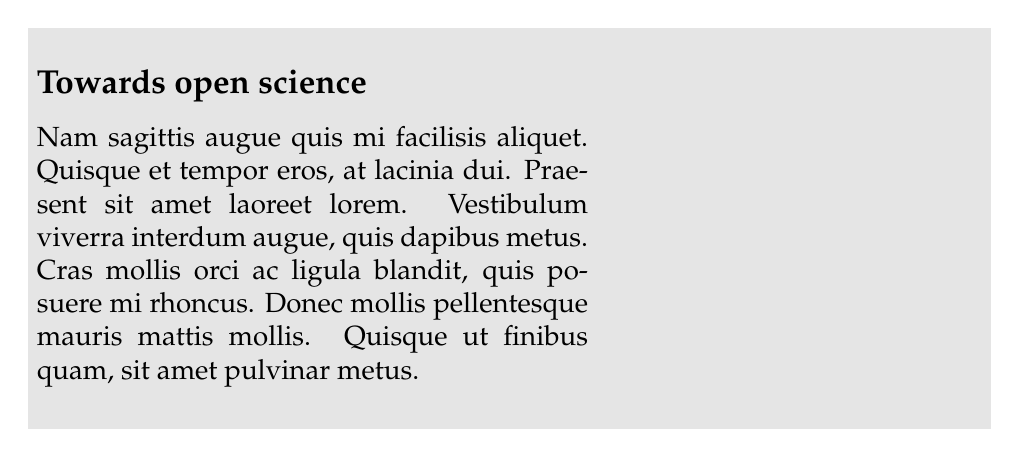
\begin{tikzpicture}[remember picture]
    %\useasboundingbox (0,0) rectangle (3,1);
    \node[xshift=2cm,yshift=7cm, fill=gray!20] at (current page.south west)
       {\begin{minipage}{12cm}
            \begin{minipage}{7cm}
            \bigskip
            \subsection*{Towards open science}

Nam sagittis augue quis mi facilisis aliquet. Quisque et tempor eros, at lacinia dui. Praesent sit amet laoreet lorem. Vestibulum viverra interdum augue, quis dapibus metus. Cras mollis orci ac ligula blandit, quis posuere mi rhoncus. Donec mollis pellentesque mauris mattis mollis. Quisque ut finibus quam, sit amet pulvinar metus.
\bigskip
            \end{minipage}
            
        \end{minipage}
       };
\end{tikzpicture}

\pagebreak


%\FloatBarrier

\section*{Contribution to Publications}
\label{ContPub}


The scientific papers that merge the core of the thesis is as follows:

\bigskip

\textbf{Paper I / Chapter 2}

\medskip

\noindent \hangindent=0.6cm Heistermann, Maik, Irene Crisologo, Catherine C. Abon, Bernard Alan Racoma, Stephan Jacobi, Nathaniel T. Servando, Carlos Primo C. David, and Axel Bronstert. 2013. “Brief Communication ‘Using the New Philippine Radar Network to Reconstruct the Habagat of August 2012 Monsoon Event around Metropolitan Manila.’” Nat. Hazards Earth Syst. Sci. 13 (3): 653–57. https://doi.org/10.5194/nhess-13-653-2013.

\medskip

MH conceptualized the study, together with IC and CCA; NTS and CPCD provided the radar data; MH wrote the software code, and MH and IC carried out the analysis. MH prepared the manuscript, with contributions from all co-authors.

\bigskip

\textbf{Paper II / Chapter 3}

\medskip

\noindent \hangindent=0.6cm Crisologo, Irene, Robert A. Warren, Kai Mühlbauer, and Maik Heistermann. 2018. “Enhancing the Consistency of Spaceborne and Ground-Based Radar Comparisons by Using Beam Blockage Fraction as a Quality Filter.” Atmospheric Measurement Techniques 11 (9): 5223–36. https://doi.org/10.5194/amt-11-5223-2018.

\medskip

IC and MH conceptualized the study. KM, MH, RW, and IC formulated the 3D-matching code based on previous work of RW. IC carried out the analyses; IC and MH the interpretation of results. IC and MH, with contributions from all authors, prepared the manuscript.

\bigskip

\textbf{Paper III / Chapter 4}

\medskip

\noindent \hangindent=0.6cm Crisologo, Irene and Maik Heistermann: Using ground radar overlaps to verify the retrieval of calibration bias estimates from spaceborne platforms, Atmos. Meas. Tech., submitted.

\medskip

IC and MH conceptualized the study and formulated the code for 3D-matching of GRs. IC prepared the scripts for 3-way comparison and carried out the analysis. IC and MH interpreted the results and prepared the manuscript. 




\end{multicols}

% Chapter 2

\chapter[Short version of title for header]{Full version of chapter title} % Main chapter title

% 

\label{Chapter2} % For referencing the chapter elsewhere, use \ref{Chapter2} 

%----------------------------------------------------------------------------------------


\noindent \rule{\textwidth}{0.4pt}

\medskip

\noindent This chapter is published as:

\medskip

\noindent \hangindent=0.6cm Heistermann, M., I. Crisologo, C. C. Abon, B. A. Racoma, S. Jacobi, N. T. Servando, C. P. C. David, and A. Bronstert. 2013. “Brief Communication ‘Using the New Philippine Radar Network to Reconstruct the Habagat of August 2012 Monsoon Event around Metropolitan Manila.’” Nat. Hazards Earth Syst. Sci. 13 (3): 653–57. https://doi.org/10.5194/nhess-13-653-2013.



\noindent\rule{\textwidth}{0.4pt}

\bigskip


\noindent \textbf{Abstract}

\medskip

\noindent
Proin maximus orci id ullamcorper blandit. Interdum et malesuada fames ac ante ipsum primis in faucibus. Mauris diam massa, sodales eu justo a, laoreet viverra quam. Vivamus vitae magna cursus, dignissim enim eget, ultrices turpis. Nunc faucibus faucibus dolor. Praesent congue fermentum viverra. Etiam venenatis ex ipsum.

%The Abstract provides a summary of the paper. It needs to be concise, because if it is not, the reader will become discouraged and will move to the next article in the journal. The abstract needs to be informative: writing ‘a theory has been presented and the implications discussed’ is simply a waste of time for everyone involved. Get straight to the facts!

\bigskip

\begin{multicols}{2}


\section{Introduction}

Nullam et semper lectus, sit amet condimentum lorem. Quisque tempus felis massa, ac molestie tellus pharetra non. Nam mollis vel urna in malesuada. Duis ultricies congue enim vitae lobortis. Maecenas consequat mi ac ligula consequat gravida. Pellentesque sed mauris iaculis, posuere dui non, porttitor turpis. Suspendisse ornare urna felis, eget luctus enim posuere quis. Pellentesque non auctor ligula. Suspendisse porta orci id ultrices facilisis.

Etiam elit mauris, mollis non nulla sit amet, porttitor dictum urna. Sed vitae volutpat nisl. Mauris egestas sollicitudin ante ut rutrum. Suspendisse non dui nec nulla tristique hendrerit quis ac eros. In porta ligula erat, blandit feugiat nulla pretium ac. In quis congue nisi, vulputate suscipit erat. Sed sit amet arcu vel ligula malesuada sollicitudin. Donec quis velit at nulla venenatis sodales ut a tellus. Phasellus semper vehicula mi, sed ultricies arcu tristique sit amet. Nullam et semper lectus, sit amet condimentum lorem. Quisque tempus felis massa, ac molestie tellus pharetra non. Nam mollis vel urna in malesuada. Duis ultricies congue enim vitae lobortis. Maecenas consequat mi ac ligula consequat gravida. Pellentesque sed mauris iaculis, posuere dui non, porttitor turpis. Suspendisse ornare urna felis, eget luctus enim posuere quis. Pellentesque non auctor ligula. Suspendisse porta orci id ultrices facilisis \citep{heistermann_technical_2013}.

% column-width figure
\noindent
\begin{minipage}[h]{0.45\textwidth}
%\centering
\includegraphics[width=\columnwidth]{./Figures/image2.jpg}
\captionof{figure}[Photo by Claudio Testa on Unsplash]{Photo by Claudio Testa on Unsplash} 
\label{fig:image2}
\end{minipage}

Proin maximus orci id ullamcorper blandit. Interdum et malesuada fames ac ante ipsum primis in faucibus. Mauris diam massa, sodales eu justo a, laoreet viverra quam. Vivamus vitae magna cursus, dignissim enim eget, ultrices turpis. Nunc faucibus faucibus dolor. Praesent congue fermentum viverra. Etiam venenatis ex ipsum. Phasellus semper tempus aliquet. Aenean id tellus condimentum, congue arcu id, bibendum odio. Praesent molestie elementum nulla. Proin ac condimentum sapien. Sed tempor orci sit amet mi luctus, eu tempus nisi pulvinar. Proin sit amet purus rutrum, accumsan ex varius, lacinia mauris. Sed sed fermentum neque. Maecenas eu vestibulum elit, ut imperdiet leo. Vestibulum tempor suscipit leo, eget interdum ligula malesuada a. Cras feugiat a nisl sit amet mattis. Vivamus varius commodo molestie \ref{fig:image2}.

Etiam elit mauris, mollis non nulla sit amet, porttitor dictum urna. Sed vitae volutpat nisl. Mauris egestas sollicitudin ante ut rutrum. Suspendisse non dui nec nulla tristique hendrerit quis ac eros. In porta ligula erat, blandit feugiat nulla pretium ac. In quis congue nisi, vulputate suscipit erat. Sed sit amet arcu vel ligula malesuada sollicitudin. Donec quis velit at nulla venenatis sodales ut a tellus. Phasellus semper vehicula mi, sed ultricies arcu tristique sit amet.


% full width figure
\begin{figure*}[ht!]
\begin{center}
\includegraphics[width=0.9\linewidth]{./Figures/image1.jpg}
\captionof{figure}[Photo by Fabian Irsara on Unsplash]{Photo by Fabian Irsara on Unsplash}
\label{fig:image1}
\end{center}
\end{figure*}


Maecenas eget placerat dolor, id suscipit nisl. Aenean consectetur faucibus iaculis. Nulla rhoncus est ligula. Duis hendrerit molestie augue, sed vehicula nisl convallis eu. Phasellus ornare augue at quam finibus porttitor vel in nunc. Proin vitae tristique erat. Donec ullamcorper quam sollicitudin leo imperdiet, sed sollicitudin odio dictum. Mauris sed tellus et ligula consectetur maximus sit amet at sem. Cras neque orci, eleifend non laoreet vel, tristique eu ante. Fusce efficitur magna vitae magna eleifend eleifend. Quisque placerat vestibulum erat eget suscipit. Vestibulum vehicula tempor justo. Morbi interdum, felis in molestie vehicula, nunc erat mollis orci, ac placerat dolor leo nec ipsum. Ut ac ultricies ex. Quisque at metus mollis, tincidunt lorem vel, sollicitudin odio. Maecenas ut nibh ac ex malesuada maximus et vel nisi.

\section{Section}

\subsection{Subsection}
\label{subsec:subsectionname2}

Use section or subsection label for reference within text \ref{subsec:subsectionname2}.

\subsubsection{Sub sub subsection}

Many many layers of sections. Soooo many layers. I think they lose numbering at this level though.

For tables following the column width, see latex code below.

% column-width table
\noindent
\begin{minipage}[t]{0.45\textwidth}
\begin{center}
\label{tab:techspecs}
\captionof{table}{Caption of table. This is a column-width table.}
\begin{tabular}{l l}
\hline
                             & Subic Radar                                                                                                    \\ \hline
Polarization                 & Single-Pol                                                                                                     \\
Position (lat/lon)           & 14.82$^{\circ} N$ 120.36 $^{\circ} E$                                                                            \\
Altitude 		             & 532 m.a.s.l.                                                                                                           \\
Maximum Range                & 120 km (150 km)                                                                                                         \\
Azimuth resolution           & 1 $^{\circ}$                                                                                                    \\
Beam width                   & 0.95 $^{\circ}$                                                                                                    \\
Gate length                  & 500 m (250 m)                                                                                                          \\
Number of elevation angles   & 14 (3)                                                                                                            \\
\hline
%Elevation angles             & \begin{tabular}[c]{@{}l@{}}0.5, 1.5, 2.4, 3.4, 4.3, 5.3, 6.2, 7.5, 8.7, 10, 12, 14, 16.7, 19.5 ($^{\circ}$) \\(0.0, 1.0, 2.0)\end{tabular} \\
Elevation angles             & 0.5, 1.5, 2.4, 3.4, 4.3, \\
& 5.3, 6.2, 7.5, 8.7, 10, \\ & 12, 14, 16.7, 19.5 ($^{\circ}$) \\ 
&(0.0, 1.0, 2.0)
\\
\hline
Volume cycle interval        & 9 minutes                                                                                                      \\
Data available since         & April 2012                                                                                                     \\
Peak power                   & 850 kW                                                                                                         \\
Wavelength                   & 10.7 cm                                                                                                        \\ \hline
\end{tabular}
\end{center}
\end{minipage}%


Proin maximus orci id ullamcorper blandit. Interdum et malesuada fames ac ante ipsum primis in faucibus. Mauris diam massa, sodales eu justo a, laoreet viverra quam. Vivamus vitae magna cursus, dignissim enim eget, ultrices turpis. Nunc faucibus faucibus dolor. Praesent congue fermentum viverra. Etiam venenatis ex ipsum.

% Full width table
\begin{table*}
\begin{center}
\caption{Caption of table. This is a full-width table.}
\begin{tabular}{@{}lcc@{}}
\toprule
                           & \multicolumn{1}{c}{Subic Radar}                  & \multicolumn{1}{c}{Tagaytay Radar}                 \\ \midrule
Bandwidth                  & S-Band                                           & C-Band                                             \\
Polarization               & Single-pol                                       & Dual-pol                                           \\
Position (lat/lon)         & 14.822°N 120.363°E                               & 14.123°N 120.974°E                                 \\
Altitude                   & 532 m a.s.l.                                     & 752 m a.s.l.                                       \\
Maximum Range              & \multicolumn{2}{c}{120 km}                                                                            \\
Azimuth Resolution         & \multicolumn{2}{c}{1 $^{\circ}$}                                                                      \\
Gate length                & \multicolumn{2}{c}{500 m}                                                                             \\
Number of elevation angles & \multicolumn{2}{c}{14}                                                                                \\
Elevation angles           & \multicolumn{2}{c}{0.5°, 1.5°, 2.4°, 3.4°, 4.3°, 5.3°, 6.2°, 7.5°, 8.7°, 10°, 12°, 14°, 16.7°, 19.5°} \\
Volume cycle interval      & 8 minutes                                        & 15 minutes                                         \\
Start of operation         & 2012                                             & 2012                                               \\ \bottomrule
\end{tabular}
\label{tab:SUBtechspecs}
\end{center}
\end{table*}%


\end{multicols}

\newpage

\section*{Supplemental material to the manuscript}

% going back to single column

Nullam et semper lectus, sit amet condimentum lorem. Quisque tempus felis massa, ac molestie tellus pharetra non. Nam mollis vel urna in malesuada. Duis ultricies congue enim vitae lobortis. Maecenas consequat mi ac ligula consequat gravida. Pellentesque sed mauris iaculis, posuere dui non, porttitor turpis. Suspendisse ornare urna felis, eget luctus enim posuere quis. Pellentesque non auctor ligula. Suspendisse porta orci id ultrices facilisis.

%
% Chapter 2

\chapter[Short version of title for header]{Full version of chapter title} % Main chapter title

% 

\label{Chapter3} % For referencing the chapter elsewhere, use \ref{Chapter3} 

%----------------------------------------------------------------------------------------


\noindent \rule{\textwidth}{0.4pt}

\medskip

\noindent This chapter is published as:

\medskip

\noindent \hangindent=0.6cm Citation



\noindent\rule{\textwidth}{0.4pt}

\bigskip


\noindent \textbf{Abstract}

\medskip

\noindent
Abstract

\bigskip

\begin{multicols}{2}


\section{Introduction}

Introduction

\section{Section}

\subsection{Subsection}
\label{subsec:subsectionname3}

Use section or subsection label for reference within text \ref{subsec:subsectionname3}.



\end{multicols}
 % paper 2

% Chapter 2

\chapter[Short version of title for header]{Full version of chapter title} % Main chapter title

% 

\label{Chapter4} % For referencing the chapter elsewhere, use \ref{Chapter4} 

%----------------------------------------------------------------------------------------


\noindent \rule{\textwidth}{0.4pt}

\medskip

\noindent This chapter is published as:

\medskip

\noindent \hangindent=0.6cm Citation



\noindent\rule{\textwidth}{0.4pt}

\bigskip


\noindent \textbf{Abstract}

\medskip

\noindent
Abstract

\bigskip

\begin{multicols}{2}


\section{Introduction}

IntroductionIntroduction Introduction IntroductionIntroduction Introduction Introduction Introduction Introduction.

\section{Section}

\subsection{Subsection}
\label{subsec:subsectionname4}

Use section or subsection label for reference within text \ref{subsec:subsectionname4}.



\end{multicols} % paper 3
%
% Chapter 5

\chapter{Discussion, Limitations, Outlook} % Main chapter title

\label{Chapter5} % For referencing the chapter elsewhere, use \ref{Chapter1} 

%----------------------------------------------------------------------------------------

% Define some commands to keep the formatting separated from the content 
%\newcommand{\keyword}[1]{\textbf{#1}}
%\newcommand{\tabhead}[1]{\textbf{#1}}
%\newcommand{\code}[1]{\texttt{#1}}
%\newcommand{\file}[1]{\texttt{\bfseries#1}}
%\newcommand{\option}[1]{\texttt{\itshape#1}}

%----------------------------------------------------------------------------------------

\begin{multicols}{2}

\noindent
Mauris justo orci, ornare vitae diam non, venenatis condimentum augue. Phasellus vestibulum, enim in pellentesque semper, ligula quam consectetur enim, quis finibus lorem tortor id nisl. Ut ultrices nibh eu augue aliquet rhoncus. Mauris tincidunt, libero ullamcorper aliquam convallis, ex tortor congue augue, ut congue odio ligula hendrerit velit. Integer finibus, sem ut interdum porttitor, neque nulla dapibus leo, at rutrum risus justo non est. Donec imperdiet porttitor augue a fringilla. Praesent suscipit sollicitudin est non eleifend. Phasellus porttitor in ex in tincidunt. Nulla facilisi. Suspendisse vestibulum fermentum fermentum. Suspendisse sagittis sit amet massa at vestibulum. Nullam quis finibus ante, elementum blandit tortor.

Maecenas eget placerat dolor, id suscipit nisl. Aenean consectetur faucibus iaculis. Nulla rhoncus est ligula. Duis hendrerit molestie augue, sed vehicula nisl convallis eu. Phasellus ornare augue at quam finibus porttitor vel in nunc. Proin vitae tristique erat. Donec ullamcorper quam sollicitudin leo imperdiet, sed sollicitudin odio dictum. Mauris sed tellus et ligula consectetur maximus sit amet at sem. Cras neque orci, eleifend non laoreet vel, tristique eu ante. Fusce efficitur magna vitae magna eleifend eleifend. Quisque placerat vestibulum erat eget suscipit. Vestibulum vehicula tempor justo. Morbi interdum, felis in molestie vehicula, nunc erat mollis orci, ac placerat dolor leo nec ipsum. Ut ac ultricies ex. Quisque at metus mollis, tincidunt lorem vel, sollicitudin odio. Maecenas ut nibh ac ex malesuada maximus et vel nisi.

Etiam elit mauris, mollis non nulla sit amet, porttitor dictum urna. Sed vitae volutpat nisl. Mauris egestas sollicitudin ante ut rutrum. Suspendisse non dui nec nulla tristique hendrerit quis ac eros. In porta ligula erat, blandit feugiat nulla pretium ac. In quis congue nisi, vulputate suscipit erat. Sed sit amet arcu vel ligula malesuada sollicitudin. Donec quis velit at nulla venenatis sodales ut a tellus. Phasellus semper vehicula mi, sed ultricies arcu tristique sit amet.

Nunc blandit auctor nulla, eu sagittis massa tempor ut. Etiam cursus justo eget nisl interdum, vitae suscipit turpis tempus. Nam tristique justo eu urna iaculis, vel ultricies nisi fringilla. Vestibulum ante ipsum primis in faucibus orci luctus et ultrices posuere cubilia Curae; Praesent nec ligula sed leo commodo aliquet. Aliquam rutrum semper mauris, sed condimentum diam faucibus ut. Cras condimentum dictum risus eget ullamcorper. Etiam varius pulvinar velit id accumsan. Aliquam ultrices, arcu ut porttitor tincidunt, tellus augue sagittis velit, non convallis turpis lacus at risus. Phasellus vel tempor risus. Proin vitae placerat orci. Phasellus blandit, est eu mattis semper, ante enim rhoncus sem, et aliquam neque neque id mauris. Ut mauris massa, suscipit eget luctus at, tincidunt at sem. Aenean in dignissim est, nec vulputate dolor.

Nullam et semper lectus, sit amet condimentum lorem. Quisque tempus felis massa, ac molestie tellus pharetra non. Nam mollis vel urna in malesuada. Duis ultricies congue enim vitae lobortis. Maecenas consequat mi ac ligula consequat gravida. Pellentesque sed mauris iaculis, posuere dui non, porttitor turpis. Suspendisse ornare urna felis, eget luctus enim posuere quis. Pellentesque non auctor ligula. Suspendisse porta orci id ultrices facilisis.



\subsection*{Limitations of the study}

Limitations of the study.

\subsection*{Outlook}

Outlook of the study. 

\end{multicols}

%Using spaceborne radar platforms to enhance the homogeneity of weather radar calibration
%
% Chapter 6

\chapter{Summary and Conclusion} % Main chapter title

\label{Chapter6} % For referencing the chapter elsewhere, use \ref{Chapter1} 

%----------------------------------------------------------------------------------------

% Define some commands to keep the formatting separated from the content 
%\newcommand{\keyword}[1]{\textbf{#1}}
%\newcommand{\tabhead}[1]{\textbf{#1}}
%\newcommand{\code}[1]{\texttt{#1}}
%\newcommand{\file}[1]{\texttt{\bfseries#1}}
%\newcommand{\option}[1]{\texttt{\itshape#1}}

%----------------------------------------------------------------------------------------
\begin{multicols}{2}

%\subsection*{Conclusion}
\noindent
The Conclusion section is an essential (and required) part of a paper: it represents what remains after the dust of the discussion has settled. No new ideas can be introduced in the Conclusions.

\end{multicols}

% Chapter 7

\chapter{Additional Publications} % Main chapter title

\label{Chapter7} % For referencing the chapter elsewhere, use \ref{Chapter1} 

%----------------------------------------------------------------------------------------

% Define some commands to keep the formatting separated from the content 
%\newcommand{\keyword}[1]{\textbf{#1}}
%\newcommand{\tabhead}[1]{\textbf{#1}}
%\newcommand{\code}[1]{\texttt{#1}}
%\newcommand{\file}[1]{\texttt{\bfseries#1}}
%\newcommand{\option}[1]{\texttt{\itshape#1}}

%----------------------------------------------------------------------------------------


I also contributed to the following publications during the course of the doctoral research, aside from the manuscripts listed in Chapter 1. 

\bigskip
\bigskip

\noindent
Bronstert, Axel, Ankit Agarwal, Berry Boessenkool, \textbf{Irene Crisologo}, Madlen Fischer, Maik Heistermann, Lisei Köhn-Reich, et al. 2018. “Forensic Hydro-Meteorological Analysis of an Extreme Flash Flood: The 2016-05-29 Event in Braunsbach, SW Germany.” Science of The Total Environment 630 (July): 977–91.\\https://doi.org/10.1016/j.scitotenv.2018.02.241.

\bigskip

\noindent
Ozturk, Ugur, Dadiyorto Wendi, \textbf{Irene Crisologo}, Adrian Riemer, Ankit Agarwal, Kristin Vogel, José Andrés López-Tarazón, and Oliver Korup. 2018. “Rare Flash Floods and Debris Flows in Southern Germany.” Science of The Total Environment 626 (June): 941–52. https://doi.org/10.1016/j.scitotenv.2018.01.172.






%----------------------------------------------------------------------------------------
%	THESIS CONTENT - APPENDICES
%----------------------------------------------------------------------------------------

%\appendix % Cue to tell LaTeX that the following "chapters" are Appendices

% Include the appendices of the thesis as separate files from the Appendices folder
% Uncomment the lines as you write the Appendices

%\include{Appendices/AppendixA}
%\include{Appendices/AppendixB}
%\include{Appendices/AppendixC}

%----------------------------------------------------------------------------------------
%	BIBLIOGRAPHY
%----------------------------------------------------------------------------------------

%\blankpage

%\newgeometry{left=3.5cm,right=2.5cm, bottom=3cm}

%\addcontentsline{toc}{chapter}{Bibliography}
\bibliographystyle{apalike}
%\ifbool{listtoc}{\addchap{Bibliography}}
%\bibliographystyle{chicago}
%\bibliographystyle{plainnat}
\setlength{\bibsep}{0.12pt plus 0.0ex}

%\begin{figure*}[ht!]
%\begin{center}
%\includegraphics[width=\linewidth]{bib_distribution.png}
%\end{center}
%\end{figure*}

%\bibliography{IreneLib}
\bibliography{ThesisTemplate}
%\restoregeometry

%%\newpage
%%\newpage
%
%\cleardoublepage
%
%\newpage
%\thispagestyle{empty}
%\mbox{}
%
%%\newpage
%%\thispagestyle{empty}
%%\AddToShipoutPicture*{\LastCoverPic} % to place the background image only in the cover page
%%\vspace*{\fill}
%%\noindent \color{white} The photo on the front-cover page shows a landslide beside a waterfall by the southwestern wall of the Aso Caldera, whereas the photo on the end-cover page is the view of the Mount Aso from the western wall of the caldera. Both the photos are taken during a field trip between 21st and 24th October, 2016.
%
%
%
%%\def\thepage{Backcover}
%%\begin{textblock*}{\paperwidth}(0pt,0pt)%
%%\noindent\includegraphics*[width=\paperwidth]{IMG_1713.JPG}
%%\end{textblock*} %\printbibliography%[heading=bibintoc]

%----------------------------------------------------------------------------------------

\end{document}  
